\chapter{Experiments}\label{chapter:experiments_and_results}
As mentioned in the previous chapter, the process of finding was an iterative one of running an experiment, analyzing the generated data, draw conclusions and then repeat the steps with a new experiments designed to amend the mistakes of the previous experiment. This chapter will go through the results that were obtained from each of the data sets. A summary and discussion of the results is found in chapter \ref{chapter:discussion}.

\section{Overview of experiments}
The model has many parameters, and doing an exhaustive search over the entire parameter space is not possible. Instead, a genetic algorithm (GA) was used to do targeted searches of the parameters. For the details of the GA, please see chapter \ref{chapter:ga}. Depending on how the GA was set up, different areas of the search space was searched. Even when using a GA, some parameters had to be fixed. However, fixing parameters means that the effect of the fixed parameter on the behavior of the model remains unknown, since only a subspace of the entire parameter space is searched. For this reason the genetic algorithm was executed several times, each creating a data set containing fitness values for different parts of the parameter space. Each of these data set can be analyzed, providing information which can be corroborated in order to form an understanding of the overall market behavior.

Table \ref{table:datasets_overview} contains an overview of the different data sets, showing which parameters were fixed, and which were included as genes in the genetic algorithm.

In the following four experiments, the genetic algorithm was set to minimize all four fitness-measures.

\begin{description}
\item[\dthree: Varying the number of HFT agents, and all latency related parameters] This data set was generated by including all the model parameters concerning time latency as well as the number of agents into the individuals in the genetic algorithm. Due to the high number of variables, the data turned out to be difficult to analyze, as too many factors pertaining to the simultaneous change of several parameters influenced the fitness values.
\item[\dnine: Fixing the number of agents while varying latency parameters] The analysis of \dthree{} showed that when minimizing the four fitness-measures, the genetic algorithm tended to select  model containing few or no HFT agents. The case of a market with no market makers and no chartists can safely be said to be trivial. Hence, in experiment \dnine, the number of HFT agents were fixed to $\ssmmnAgents = 30$ and $\scnAgents = 100$.
\item[\dten: Fixing the number of HFT chartists] Since \dnine kept \ssmmnAgents and \scnAgents constant, the experiment did not reveal anything on how the market behavior changes when the number of agents changes. In order to investigate the impact of having many or few HFT market makers, \ssmmnAgents was varied in this experiment. Although it is also of interest how the market behavior depends on the number of HFT chartists, including \scnAgents as a gene would yield results similar to those obtained in \dthree. For this reason the number of HFT chartists was fixed to $\scnAgents = 150$.
\item[\deleven: Fixing the number of HFT market makers] This experiment was carried out in order to investigate the impact of the number of HFT chartists on the market behavior, and is supplementary to \dten.
\end{description}


\begin{table}
\begin{tabular}{|l|L|E|L|}
\toprule
ID & Description & Fixed parameters& As genes \\
\midrule
\dthree & All parameters varied& $\scordervolumemu=10$,$\scordervolumes=3$,$\ssmmordervolumemu=50$,$\ssmmordervolumes=20$,$\scticksbeforereactingmu=2$,$\scticksbeforereactings=5$,$\scpriceticksizemu=3$,$\scpriceticksizes=2$ &  \sclatencymu, \sclatencys, \scnAgents, \scthinkmu, \scthinks, \sctimehorizonmu, \sctimehorizons, \scwaitTimeBetweenTradingmu, \scwaitTimeBetweenTradings, \ssmmlatencymu, \ssmmlatencys, \ssmmnAgents, \ssmmthinkmu, \ssmmthinks\\
\midrule
\dnine & Fixed number of HFT agents &$\ssmmnAgents = 30$, $\scnAgents = 100$,$\scordervolumemu=10$,$\scordervolumes=3$,$\ssmmordervolumemu=50$,$\ssmmordervolumes=20$,$\scticksbeforereactingmu=2$,$\scticksbeforereactings=5$,$\scpriceticksizemu=3$, $\scpriceticksizes=2$ & \scthinkmu, \scthinks, \sctimehorizonmu, \sctimehorizons, \scwaitTimeBetweenTradingmu, \scwaitTimeBetweenTradings, \ssmmlatencymu, \ssmmlatencys, \ssmmnAgents, \ssmmthinkmu, \ssmmthinks \\
\midrule
\dten & Fixed number of HFT chartists and fixed strategy parameters & $\scnAgents = 150$, $\ssmmthinkmu = \scthinkmu = 50$, $\ssmmthinks = \scthinks = 20$, $\sctimehorizonmu = 5000$, $\sctimehorizons = 2000$, $\scwaitTimeBetweenTradingmu = 50$, $\scwaitTimeBetweenTradings = 20$,$\scordervolumemu=10$,$\scordervolumes=3$,$\ssmmordervolumemu=50$,$\ssmmordervolumes=20$,$\scticksbeforereactingmu=2$,$\scticksbeforereactings=5$, $\scpriceticksizemu=3$,$\scpriceticksizes=2$  & \ssmmnAgents, \sclatencymu, \sclatencys, \ssmmlatencymu, \ssmmlatencys \\
\midrule
\deleven & Fixed number of HFT market makers and fixed strategy parameters & $\ssmmnAgents = 52$, $\ssmmthinkmu = \scthinkmu = 50$, $\ssmmthinks = \scthinks = 20$, $\sctimehorizonmu = 5000$, $\sctimehorizons = 2000$, $\scwaitTimeBetweenTradingmu = 50$, $\scwaitTimeBetweenTradings = 20$,$\scordervolumemu=10$,$\scordervolumes=3$,$\ssmmordervolumemu=50$,$\ssmmordervolumes=20$,$\scticksbeforereactingmu=2$,$\scticksbeforereactings=5$, $\scpriceticksizemu=3$,$\scpriceticksizes=2$  & \ssmmnAgents, \sclatencymu, \sclatencys, \ssmmlatencymu, \ssmmlatencys \\
\bottomrule
\end{tabular}
\caption{Overview of datasets}
\label{table:datasets_overview}
\end{table}




\section{Data distribution}
The quickest way to get an idea of how the data generated by the simulations is distributed is to make scatter plots. The data of the model fitness is four-dimensional, requiring twelve plots to visualize all combinations. However, since \overshoot is discrete with a small range of values, it is not suitable for a scatter plot. Furthermore, some scatter plots are not useful for interpretation if they do not show any structure in the data. Figure \ref{figure:d9_scatter_fitness} shows three scatter plots which were found to best illustrate the structure of the dataset from \dnine. Note also that coloring each point corresponding to its value in one dimension makes it possible to show how the data is distributed in three dimensions.
\begin{figure}
\centering
\subcaptionbox{$\log \stdev$ vs. $\log \roundstable$ vs. \timetoreachnewfundamental}
[0.49\linewidth]{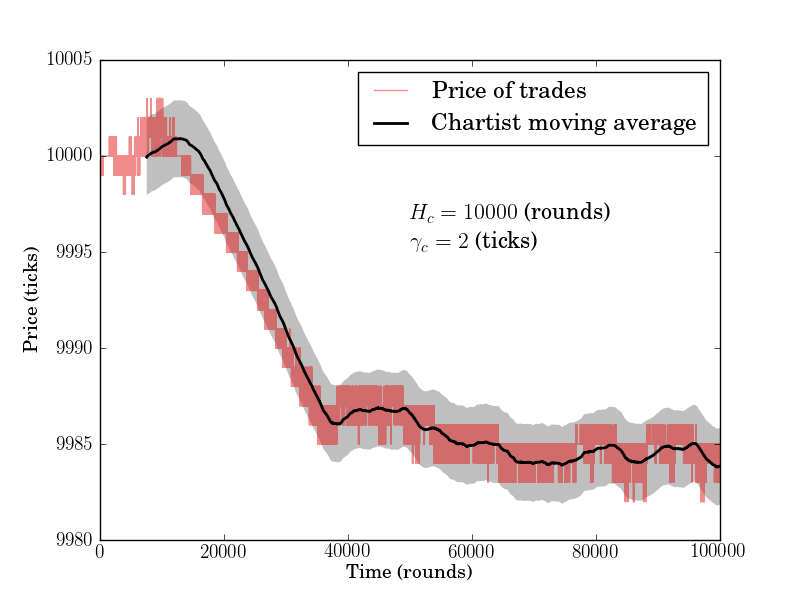
\includegraphics[width=0.5\textwidth]{21_scatter_plots/d9/d.png}}
\subcaptionbox{\roundstable vs. \timetoreachnewfundamental vs. \stdev}
[0.49\linewidth]{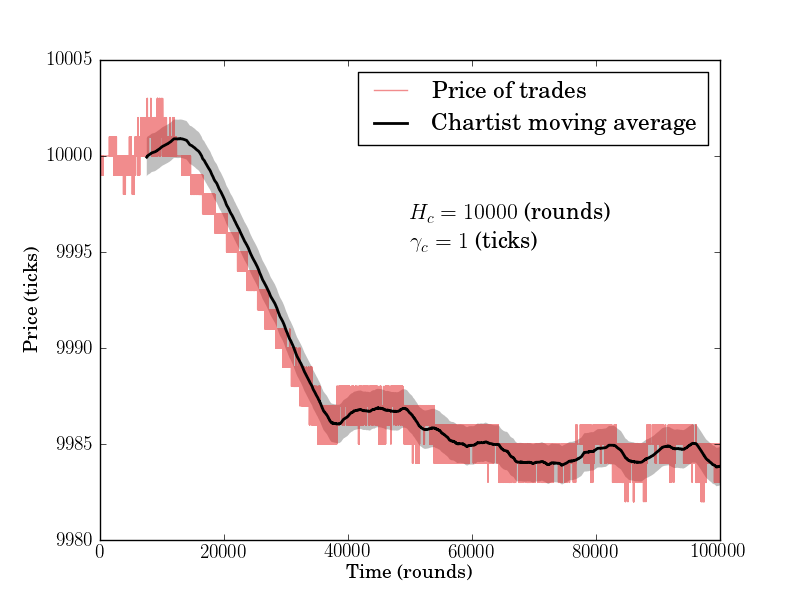
\includegraphics[width=0.5\textwidth]{21_scatter_plots/d9/c.png}}
\subcaptionbox{$\log \overshoot$ vs . $\log \stdev$ vs. \timetoreachnewfundamental}
[0.49\linewidth]{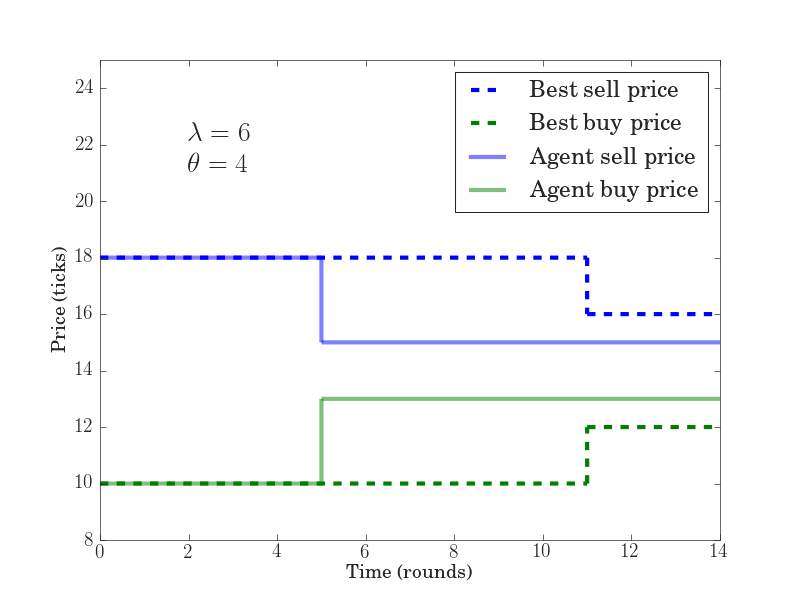
\includegraphics[width=0.5\textwidth]{21_scatter_plots/d9/b.png}}
\caption{Scatter plots of fitness measures in experiment \dnine. }
\label{figure:d9_scatter_fitness}
\end{figure}
The scatter plots do seem to reveal some structure, the presence of large values in the \stdev feature obscures the nature of this structure, in spite of the logarithmic scaling. The plot showing $\log \stdev$ vs. $\log \roundstable$ is squeezed to the left, and the color grading on the scatter plot for $\log \overshoot$ vs . $\log \stdev$ reveals no variety in the \stdev feature. In an attempt to get some more information out of the scatter plot, data points with an overshoot of over 100 \% of the shock to the fundamental (corresponding to $\overshoot > 10$ ) are removed. The resulting scatter plots for the reduced data set are shown on figures \ref{figure:scatter_fitness_inliers_a} and \ref{figure:scatter_fitness_inliers_b}.

First of all, it is seen that while the data is distributed similarly in the three data sets, there are some differences. The data from \dnine{} seems to have many ``lonely'' data points, which are not part of any cluster, whereas the data from \dten{} somehow seems to be the cleanest of the three. In all three data sets, there are clusters of data. The clusters do not necessarily mean anything in themselves. They might simply be due to the way that data points are mutated and crossed by the GA. However, by considering which regions of the fitness space that each cluster covers, it is possible to add meaning to the clusters in terms of model behavior.

\begin{figure}
\centering
\subcaptionbox{Experiment \dnine}[0.49\linewidth]{\includegraphics[width=0.5\textwidth]{103_scatter_manual_outlier/d9/f.png}}
\subcaptionbox{Experiment \dnine}[0.49\linewidth]{\includegraphics[width=0.5\textwidth]{103_scatter_manual_outlier/d9/j.png}}
\subcaptionbox{Experiment \dten}[0.49\linewidth]{\includegraphics[width=0.5\textwidth]{103_scatter_manual_outlier/d10/f.png}}
\subcaptionbox{Experiment \dten}[0.49\linewidth]{\includegraphics[width=0.5\textwidth]{103_scatter_manual_outlier/d10/j.png}}
\subcaptionbox{Experiment \deleven}[0.49\linewidth]{\includegraphics[width=0.5\textwidth]{103_scatter_manual_outlier/d11/f.png}}
\subcaptionbox{Experiment \deleven}[0.49\linewidth]{\includegraphics[width=0.5\textwidth]{103_scatter_manual_outlier/d11/j.png}}
\caption{Scatter plot of \roundstable against \timetoreachnewfundamental with coloring showing $\log \stdev$ and \overshoot}
\label{figure:scatter_fitness_inliers_a}
\end{figure}

\begin{figure}
\centering
\subcaptionbox{Experiment \dnine}[0.49\linewidth]{\includegraphics[width=0.5\textwidth]{103_scatter_manual_outlier/d9/h.png}}
\subcaptionbox{Experiment \dnine}[0.49\linewidth]{\includegraphics[width=0.5\textwidth]{103_scatter_manual_outlier/d9/k.png}}
\subcaptionbox{Experiment \dten}[0.49\linewidth]{\includegraphics[width=0.5\textwidth]{103_scatter_manual_outlier/d10/h.png}}
\subcaptionbox{Experiment \dten}[0.49\linewidth]{\includegraphics[width=0.5\textwidth]{103_scatter_manual_outlier/d10/k.png}}
\subcaptionbox{Experiment \deleven}[0.49\linewidth]{\includegraphics[width=0.5\textwidth]{103_scatter_manual_outlier/d11/h.png}}
\subcaptionbox{Experiment \deleven}[0.49\linewidth]{\includegraphics[width=0.5\textwidth]{103_scatter_manual_outlier/d11/k.png}}
\caption{Scatter plot of $\log \stdev$ against \timetoreachnewfundamental with coloring showing $\roundstable$ and \overshoot}
\label{figure:d9_scatter_fitness_inliers_b}
\end{figure}
\subsection{Manually grouping simulations by behavior}
Table \ref{table:manual_filtering} contains an overview of the named criteria used for roughly grouping simulations into different types of behavior. The following text contains the reasoning for why each of these groups are interesting.

In figure \ref{figure:scatter_fitness_inliers_a}, the black dashed lines at $\timetoreachnewfundamental = \roundstable$ divide each plot into region A, (upper left triangle) and region B (lower right triangle). Region A contains the fitness-points of the simulations which are counted as stable \textit{after} they reach the new fundamental, and region B contain those that become stable before. 

\subsubsection*{Fast and stable simulations with flickering prices}
The points in the lower left corner in are those which quickly reached the new fundamental price, and quickly because stable, leading those simulations to be assigned low \timetoreachnewfundamental and \roundstable fitness-values. These points are extracted by using filter F1 (see table \ref{table:manual_filtering})

\subsubsection*{Slow or fast and stable simulations with non-flickering prices}
All three data sets have data points which are close to the diagonal. However, only \dnine{} has data points which are close to the diagonal in the upper right corner of the figure. These points are interesting because they belong to simulations which became stable as soon as they reached the new fundamental price. Hence, these simulations should have prices that do not flicker, and therefore yield a small \stdev-fitness. This is confirmed by looking at the left scatter plot of \dnine, as all the points close to the dotted line has a green/blue color. The right plot of \dnine{} shows that these simulations did not have any overshoot. It is interesting that both slow simulations which take a long time to reach the new fundamental, as well as simulations who manage to be fast, have no overshoot, and this observation begs the question of whether or not these simulations have some common parameters that make them behave in such a way. These points are extracted by applying filters F2 and F3 (see table \ref{table:manual_filtering}) to the data matrix \datamatrixfit{\dnine} which selects points that lie within a distance of 400 rounds of the diagonal. 


\subsubsection*{Stable before reaching the new fundamental}
Most of the simulations falling in region B, meaning that they became stable before reaching the new fundamental price, had no overshoot. However, when the model was allowed to have a large number of chartists, but in \deleven, a group of simulations did have a small overshoot. These two groups of points were extracted by applying filters F4 and F5  (see table \ref{table:manual_filtering}).

\subsubsection*{Simulations with overshoot}
F6

\subsubsection{Fast simulations}
All three experiments produces a group of simulations which had a quick response to the shock, but took longer to become stable. The simulations are in the column-shaped cluster in figure \ref{figure:scatter_fitness_inliers_a} and the all have relatively low \timetoreachnewfundamental-fitness of less than 25000 rounds or so. These data points were extracted using filters F7 and F8 (see table \ref{table:manual_filtering}).
\subsubsection*{Unstable simulations with non-flickering prices}
F9
The final group of simulation that are singles out in this section are those that had very smooth price curves (that is, a small value for \stdev), yet did not manage to become stable.

\begin{figure}
\centering
\subcaptionbox{Experiment \dnine}[0.32\linewidth]{\includegraphics[width=0.32\textwidth]{manual_filtering/d9/group_overlap.png}}
\subcaptionbox{Experiment \dnine}[0.32\linewidth]{\includegraphics[width=0.32\textwidth]{manual_filtering/d10/group_overlap.png}}
\subcaptionbox{Experiment \dten}[0.32\linewidth]{\includegraphics[width=0.32\textwidth]{manual_filtering/d11/group_overlap.png}}
\caption{Jaccard index between the sets of data points extracted by each filter}
\label{figure:jaccard_index}
\end{figure}

The criteria in table \ref{table:manual_filtering} do not prevent a simulation to be selected by different filters. The groups of points are therefore likely to have a non-empty intersection. Using the filters is an the attempt to separate the simulations by their behavior. Hence, the filters should in general not select the same data points. The Jaccard index $J(A,B)$ is calculated between sets $A$ and $B$ and used to determine the overlap between the sets.
\begin{equation}
J(A,B) = \frac{\lVert A \cap B \rVert}{\lVert A \cup B\rVert }
\end{equation}

\begin{equation}
J(A,B) = \frac{\lVert A \cap B \rVert}{\min \lVert A \rVert, \lvert B\rVert }
\end{equation}
Figure \ref{figure:jaccard_index}

\begin{table}
\centering
\begin{tabular}{l|E|l|E}
\toprule
ID & Target simulations & Filter criteria\\
\midrule
F1 & Fast and stable (but maybe flickering) & $\timetoreachnewfundamental < 12000$, $\roundstable < 12000$, $\log \stdev > 0$ \\
\midrule
F2 & Slow, stable and not flickering (diagonal)& $\lvert \timetoreachnewfundamental - \roundstable \rvert < 400$\\
\midrule 
F3 & Fast and stable and not flickering (diagonal)& $\lvert \timetoreachnewfundamental - \roundstable \rvert < 400$\\
\midrule
F4 & Stable before reaching fundamental, no overshoot& $\roundstable < \timetoreachnewfundamental$, $\overshoot = 0$\\
\midrule
F5 & Stable before reaching fundamental, with overshoot& $\roundstable < \timetoreachnewfundamental$, $\overshoot = >$\\
\midrule
F6 & Has overshoot & $\roundstable > \timetoreachnewfundamental$, $\overshoot > 0$ \\
\midrule
F7 & Fast response, quick to stabilize & $1000 < \timetoreachnewfundamental < 25000$, $20000 < \roundstable < 40000$ \\
\midrule
F8 & Fast response, slow to stabilize & $1000 < \timetoreachnewfundamental < 25000$, $40000 < \roundstable < 75000$ \\
\midrule
F9 & Smooth prices with a small overshoot, yet unstable & $e^{-0.5} - 0.1 < \log \stdev < e^{-0.5} + 0.1$ \\
\midrule
\bottomrule
\end{tabular}
\caption{Filter IDs and fitness-regions}
\label{table:manual_filtering}
\end{table}

\begin{table}
 \centering
 \begin{tabular}{lrrrrrrrrr}
\toprule
{} &      F1 &      F2 &      F3 &      F4 &      F5 &      F6 &      F7 &      F8 &      F9 \\
\midrule
\sclatencymu                 &    70.1 &    65.5 &    49.5 &    81.5 &    76.7 &    58.5 &    75.8 &    75.6 &    76.0 \\
 \sclatencys                 &     5.4 &     5.5 &     7.8 &     4.5 &     4.9 &     6.8 &     5.0 &     4.9 &     5.0 \\
 \scthinkmu                  &    59.7 &    58.8 &    51.8 &    70.1 &    65.8 &    53.5 &    65.7 &    64.8 &    65.9 \\
 \scthinks                   &    12.0 &    12.0 &    12.8 &    11.2 &    11.6 &    11.2 &    11.4 &    11.6 &    11.6 \\
 \sctimehorizonmu            &  1744.0 &  1676.1 &  1758.1 &  1766.8 &  1773.6 &  1906.9 &  1795.3 &  1757.2 &  1777.9 \\
 \sctimehorizons             &  1483.2 &  1472.7 &  1573.4 &  1415.7 &  1444.2 &  1346.7 &  1437.3 &  1442.4 &  1465.4 \\
 \scwaitTimeBetweenTradingmu &    29.5 &    27.4 &    29.3 &    30.5 &    30.0 &    28.6 &    30.0 &    29.7 &    29.9 \\
 \scwaitTimeBetweenTradings  &     3.2 &     4.1 &     4.2 &     3.0 &     3.1 &     5.1 &     3.1 &     3.0 &     3.1 \\
 \ssmmlatencymu              &    45.2 &    38.5 &    37.6 &    49.8 &    47.3 &    39.2 &    46.1 &    46.3 &    44.5 \\
 \ssmmlatencys               &     4.2 &     4.9 &     4.6 &     4.3 &     4.4 &     5.4 &     4.1 &     4.2 &     5.1 \\
 \ssmmthinkmu                &    39.8 &    38.2 &    40.1 &    37.9 &    38.6 &    35.5 &    39.0 &    39.1 &    35.5 \\
 \ssmmthinks                 &     0.0 &     0.0 &     0.0 &     0.0 &     0.0 &     3.6 &     0.0 &     0.3 &     0.2 \\
\overshoot                   &     1.0 &     1.1 &     1.3 &     0.0 &     1.0 &     3.9 &     1.9 &     2.1 &     1.4 \\
 \roundstable                & 11712.3 & 44993.4 & 13454.5 & 13121.9 & 13468.1 & 80410.6 & 26840.4 & 61259.6 & 54143.9 \\
 \stdev                      &     1.2 &     0.7 &     0.7 &     0.6 &     0.7 &     1.1 &     0.8 &     0.9 &     0.6 \\
 \timetoreachnewfundamental  & 13767.0 & 45089.4 & 13579.4 & 15564.3 & 16743.6 & 16513.3 & 17502.8 & 16812.7 & 40564.2 \\
Count                        &   498.0 &    33.0 &  1031.0 & 33928.0 & 41982.0 & 30468.0 &  2016.0 &  1733.0 &  2160.0 \\
\bottomrule
\end{tabular}
 \label{table:manual_filtering_d9}
 \caption{XXX}
 \end{table}
\begin{table}
 \centering
 \begin{tabular}{lrrrrrrrrr}
\toprule
{} &      F1 &  F2 &  F3 &      F4 &      F5 &      F6 &      F7 &      F8 &      F9 \\
\midrule
\sclatencymu                &   103.0 & N/A & N/A &   123.8 &   121.5 &    78.3 &   116.9 &   104.2 &    95.0 \\
 \sclatencys                &    13.0 & N/A & N/A &     6.5 &     6.5 &     9.0 &     7.1 &     8.7 &     8.7 \\
 \ssmmlatencymu             &    88.0 & N/A & N/A &    73.9 &    75.8 &    39.2 &    73.3 &    59.6 &    35.9 \\
 \ssmmlatencys              &     3.0 & N/A & N/A &     5.6 &     6.0 &     9.6 &     6.6 &     8.7 &     9.2 \\
 \ssmmnAgents               &   120.0 & N/A & N/A &   126.5 &   125.6 &    67.1 &   121.2 &    98.0 &    81.2 \\
\overshoot                  &     1.0 & N/A & N/A &     0.0 &     1.0 &     4.1 &     1.8 &     2.1 &     0.2 \\
 \roundstable               & 12260.0 & N/A & N/A & 17025.9 & 15920.1 & 81539.2 & 27387.5 & 59444.5 & 24392.3 \\
 \stdev                     &     1.0 & N/A & N/A &     0.6 &     0.7 &     1.2 &     0.7 &     0.9 &     0.6 \\
 \timetoreachnewfundamental & 14402.0 & N/A & N/A & 20405.2 & 18724.9 & 15504.3 & 18725.1 & 16840.5 & 31017.6 \\
Count                       &     1.0 & 0.0 & 0.0 &  8486.0 & 25574.0 & 47493.0 &  5379.0 &  2528.0 &   399.0 \\
\bottomrule
\end{tabular}
 \label{table:manual_filtering_d10}
 \caption{XXX}
 \end{table}
\begin{table}
 \centering
 \begin{tabular}{lrrrrrrrrr}
\toprule
{} &      F1 &  F2 &  F3 &      F4 &      F5 &      F6 &      F7 &      F8 &      F9 \\
\midrule
\sclatencymu                &    30.5 & N/A & N/A &    30.4 &    32.3 &    33.3 &    34.3 &    35.1 &    35.8 \\
 \sclatencys                &     4.8 & N/A & N/A &     9.3 &     9.9 &     4.6 &     7.2 &     6.6 &     9.0 \\
 \scnAgents                 &    39.0 & N/A & N/A &    19.0 &    26.9 &   154.0 &    46.3 &    54.6 &    41.1 \\
 \ssmmlatencymu             &    16.8 & N/A & N/A &    67.2 &    55.0 &    38.9 &    50.0 &    47.3 &    46.0 \\
 \ssmmlatencys              &    25.3 & N/A & N/A &     8.4 &    11.6 &    22.9 &    17.5 &    19.5 &    14.7 \\
\overshoot                  &     1.0 & N/A & N/A &     0.0 &     1.0 &    14.6 &     2.0 &     2.6 &     0.0 \\
 \roundstable               & 11124.3 & N/A & N/A & 15678.2 & 15075.3 & 87971.4 & 31954.9 & 63613.9 & 21851.4 \\
 \stdev                     &     1.0 & N/A & N/A &     0.7 &     0.8 &     3.6 &     0.9 &     1.0 &     0.6 \\
 \timetoreachnewfundamental & 14088.3 & N/A & N/A & 19965.3 & 18765.4 & 13685.0 & 17265.5 & 16449.5 & 31048.9 \\
Count                       &     4.0 & 0.0 & 0.0 & 71329.0 & 31377.0 & 84597.0 &   349.0 &  3014.0 &  1706.0 \\
\bottomrule
\end{tabular}
 \label{table:manual_filtering_d11}
 \caption{XXX}
 \end{table}



 

\begin{enumerate}
\item In figure \ref{figure:d9_scatter_fitness_inliers_t_r_logs}, the density of points is slightly higher around the region defined by $\roundstable = \timetoreachnewfundamental$. This is true both for small and large values of \timetoreachnewfundamental and \roundstable. Furthermore, these points all have small values for $\stdev$. The same points can be identified by looking at figure \ref{figure:d9_scatter_fitness_inliers_a}, where a cloud of points lay around the vertical line $\log \stdev \approx -0.6$.
\begin{enumerate}
	\item The low \stdev means that the traded price is stable after entering the stability margin. Furthermore, the simulations represented by these same points are among the ones with the most stable traded prices.
	%\item Because of the high correlation between \stdev and \overshoot, simulations belonging to this group have little or no overshoot. 
	\item Since $\timetoreachnewfundamental \approx \roundstable$, the traded does not leave the stability margin once it has entered. This is true for both small and large values of \timetoreachnewfundamental and \roundstable.
\end{enumerate}
\item In figure \ref{figure:d9_scatter_fitness_inliers_t_r_logs} The density seems high in the region defined by the inequalities $0.2 < \timetoreachnewfundamental < 0.3$ and $\roundstable > 0.25$. 
	\begin{enumerate}
	\item Simulations in this group reach the new fundamental quickly (less than $2\cdot 10^4$ rounds after the shock), but then leave the stable region again.
	\item The simulations which take a longer time to become stable also have less stable traded prices (higher values of \stdev)
	\end{enumerate}
\end{enumerate}



\subsubsection{\stdev vs. \timetoreachnewfundamental}



\begin{enumerate}
\item The two large clusters of red points in figure \ref{figure:d9_scatter_fitness_inliers_c} are all the simulations which never became stable during the simulation. The horizontal cluster contain the simulations which responded quickly to the shock by taking only between 10.000 and 20.000 rounds. This cluster contains simulations with both high and low \stdev values, indicating varied behavior.
\item The spike of points on the right side of the cluster are simulations that did become stable, but did so slowly and with no overshoot, as is seen by observing that all the points in the cluster are blue when the color indicated the value of \overshoot as in figure \ref{figure:d9_scatter_fitness_inliers_logs_t_o}.
\end{enumerate}





